\documentclass{article}

\usepackage[top= 27mm, bottom=27mm, left=25mm, right=25mm]{geometry}
\usepackage{graphicx}
\usepackage[unicode]{hyperref}
\usepackage{float}
\usepackage{booktabs,hhline}
\usepackage{caption}
\usepackage{subcaption}
\usepackage[english,serbian]{babel}
\usepackage[T2A]{fontenc} % enable Cyrillic fonts
\usepackage[utf8]{inputenc} % make weird characters work
\usepackage[T1]{fontenc}
\graphicspath{ {./slike/} }

\renewcommand{\figurename}{Slika}
\renewcommand{\contentsname}{Sadr\v{z}aj}

\hypersetup{
    colorlinks=true,
    linktoc=all,     %linkovi ka svim odeljcima
    linkcolor=blue,
}

\begin{document}

\begin{titlepage}

\newcommand{\HRule}{\rule{\linewidth}{0.5mm}}
\center
\textup{\Large Univerzitet u Beogradu\\Matemati\v cki fakultet}\\[1.5cm]
\textup{\Large Projekat iz Infomacionih sistema}\\[0.4cm]

\HRule \\[0.4cm]
{ \huge \bfseries Informacioni sistem za CarGo aplikaciju}\\[0.4cm]
\HRule \\[8.5cm]

\begin{minipage}{0.4\textwidth}
\begin{flushleft}
\large
\emph{Autori:}\\
\textup Luka Banduka\\
\textup Filip Jovašević\\
\textup Igor Mandić\\
\textup Nenad Perišić\\
\textup Stefan Lazović\\
\textup David Šćepanović

\end{flushleft}
\end{minipage}
\hfill
\begin{minipage}{0.4\textwidth}
\begin{flushright}
\large
\emph{Profesor:} \\
\textup Saša Malkov\\
\end{flushright}
\end{minipage}\\[2cm]


{\textup \large \today}\\[1cm]

\end{titlepage}

\newpage
\tableofcontents

\newpage
\section{\bfseries Uvod}


\section{\bfseries Analiza sistema}

OVDE CODA PISE
     
\subsection{\bfseries Dijagram konteksta celog sistema}

\quad Na slici \ref{fig:contextDiagram} prikazani su dijagram konteksta i akteri, a na slici \ref{fig:dtp1} je dat DTP dijagram nivoa jedan.
\paragraph{Registrovanje korisnika:}
    Da bi korisnik mogao da se prijavi prvo biti registrovan. Registraciju obavlja sam i dobija odgovor na kraju da li je uspe\v sno registrovan ili ne.
\paragraph{Login korisnika:}
    Da bi korisnik mogao da zatra\v zi vo\v znju mora biti prijavljen. On to radi samostalno i kao odgovor dobija da li se uspe\v sno prijavio.
\paragraph{Rad sa voza\v cima:}
    Uslov da bi voza\v c mogao da vozi korisnike je da on bude registrovan. Proces registracije obavlja uspomo\' c HR slu\v zbe. Tako\dj e voza\v c, ukoliko nije pogodan, mo\v ze biti obrisan iz sistema i samim tim mu biti zabranjeno da dalje prevozi korisnike. Taj posao obavlja HR. Ukoliko novoregistrovani voza\v c nema svoje vozilo HR pravi zahtev \v sefu voznog parka i daje na kori\v scenje voza\v cu.
\paragraph{Login voza\v ca:}
    Kako bi mogao da prevozi korisnike, voza\v c prvo mora da se prijavi. On to radi samostalno i kao odgovor dobija da li se uspe\v sno prijavio.
\paragraph{Vo\v znja:}
    Korisnik napravi zahtev za vo\v znju, slobodan voza\v c prihvati. Voza\v c do\dj e na dogovorenu lokaciju i preveze korisnika na \v zeljeno mesto. Korisnik na jedan od dva ponu\dj ena na\v cina plati vo\v znju i opciono oceni voza\v ca.
\paragraph{Nabavka vozila:}
    U sistemu postoje dve vrste voza\v ca. Voza\v ci koji imaju svoj automobil i oni koji dobijaju automobil na kori\v s\' cenje prilikom registracije. Da se ne bi desilo da nema slobodnih automobila za novoregistrovanog voza\v ca, \v sef voznog parka obavlja nabavku novih automobila.

\begin{figure}[H]
\begin{center}
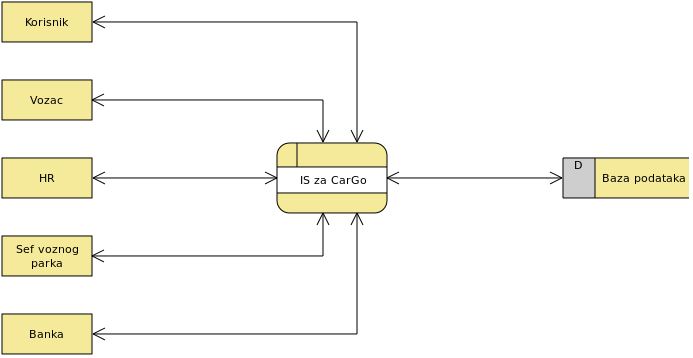
\includegraphics[width=\textwidth]{CarGoContextDiagram.png}
\end{center}
    \caption{Dijagram konteksta celog infomacionog sistema.}
\label{fig:contextDiagram}
\end{figure}

\begin{figure}[H]
\begin{center}
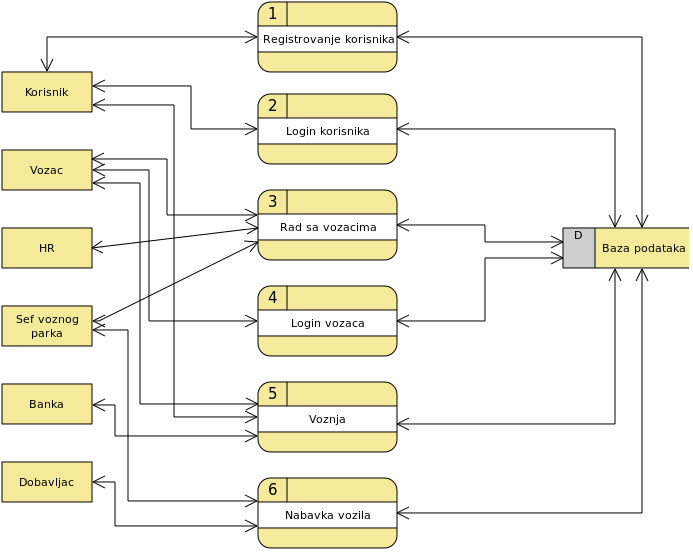
\includegraphics[width=\textwidth]{ISzaCarGo.png}
\end{center}
    \caption{DTP dijagram sistema nivoa 1.}
\label{fig:dtp1}
\end{figure}

\subsection{\bfseries Akteri}

OVDE AKTERI

\section{\bfseries Slu\v cajevi upotrebe}

\subsection{\bfseries Registrovanje korisnika}
\subsection{\bfseries Login korisnika}
\subsection{\bfseries Rad sa vozačima}
\subsubsection{\bfseries Registrovanje vozača}
\subsubsection{\bfseries Zahtev za automobil}
\subsubsection{\bfseries Otpuštanje vozača}
\subsection{\bfseries Login vozača}
\subsection{\bfseries Vožnja}
\subsubsection{\bfseries Naručivanje vožnje}
\subsubsection{\bfseries Prihvatanje vožnje}
\subsubsection{\bfseries Prevoz putnika}
\subsubsection{\bfseries Ocenjivanje voza\v ca}
\subsubsection{\bfseries Naplata vo\v znje}
\subsection{\bfseries Nabavka vozila}
\subsubsection{\bfseries Kreiranje narud\v zbine vozila}
\subsubsection{\bfseries Upravljanje podacima o dobavlja\v cima}
\subsubsection{\bfseries Prijem pristiglih vozila}

\end{document}